\section*{Introduction}

% DSBs are a serious threat to cells
% They can occur from different sources
% Different break mechanisms can result in different RecBCD substrates, and slightly different repair mechanisms
DNA double-strand breaks (DSBs) pose a serious threat to the integrity of bacterial cells. They can arise from various sources such as gamma radiation, antibiotic exposure, or collision of the replication fork with DNA-bound proteins. In \emph{E. coli}, DSB repair is initiated by the RecBCD complex. However, different sources of DSBs can lead to slightly different repair pathways, as illustrated on Figure \ref{Fig:DSB_scheme}.

In the case of a two-sided DSB (created for example by radiation or antibiotics), the break is first recognised by the RecBCD complex, which will bind to it and start translocating along the DNA at a speed of $\sim$1.5 kb/s, thanks to its combined 5' and 3' helicase activities. While translocating, RecBCD will digest both DNA strands until it meets a specific 8-base pair sequence (5'-GCTGGTGG-3') called Chi-site. Upon recognition of the Chi-site, RecBCD will pause briefly before resuming translocation, albeit with modified nuclease activity: the 5' DNA end will be degraded more slowly, and the 3' end will not be degraded at all, leading to a 3' DNA overhang. Of note, Chi recognition by RecBCD is not systematic, and will only occur with a $\sim$XX\% probability. As RecBCD creates the 3' overhang, the nuclease domain of its RecB subunit will promote loading of the RecA protein onto the single-stranded DNA. The resulting RecA-DNA nucleoprotein filament will be used as a template to search for an intact homologous sequence and perform homologous recombination.

A frequent cause of DSBs in \emph{E. coli} is replication fork collisions, which has been reported to occur in $\sim$18\% of cells per cell cycle.\cite{Sinha2018} When the replication fork collides with a DNA-bound protein, it can provoke the disassembly of the replisome. The resulting Y-shaped DNA structure is then bound by the RuvAB complex, which will pull the DNA strands (in a process called "branch migration") to create a "chicken-foot" four-way DNA structure. The free end of this structure (DNA tail) is bound by RecBCD, which will either (i) digest the whole DNA tail and displace RuvAB, allowing the replisome to be re-loaded, or (ii) recognise a Chi-site and load the RecA protein onto the 3' end of the DNA tail. Since this part of the DNA was recently replicated, a homologous sequence is necessarily present in close proximity, and can be used for homologous recombination.

In the case of fork collisions, the DSB repair process is expected to occur faster than in the case of a two-sided break caused by antibiotics or radiation. Since the DNA tail is only a few kilobases long, its full digestion by RecBCD would only take a few seconds, and if a Chi-site is recognised and RecA loaded, the close proximity of a homologous sequence should ensure rapid homology searching. In the case of a two-sided break however the homologous sequence is not guaranteed to be nearby, and the homology search can take several minutes.\cite{Wiktor2021}

\begin{figure*}[htbp]
    \centering
    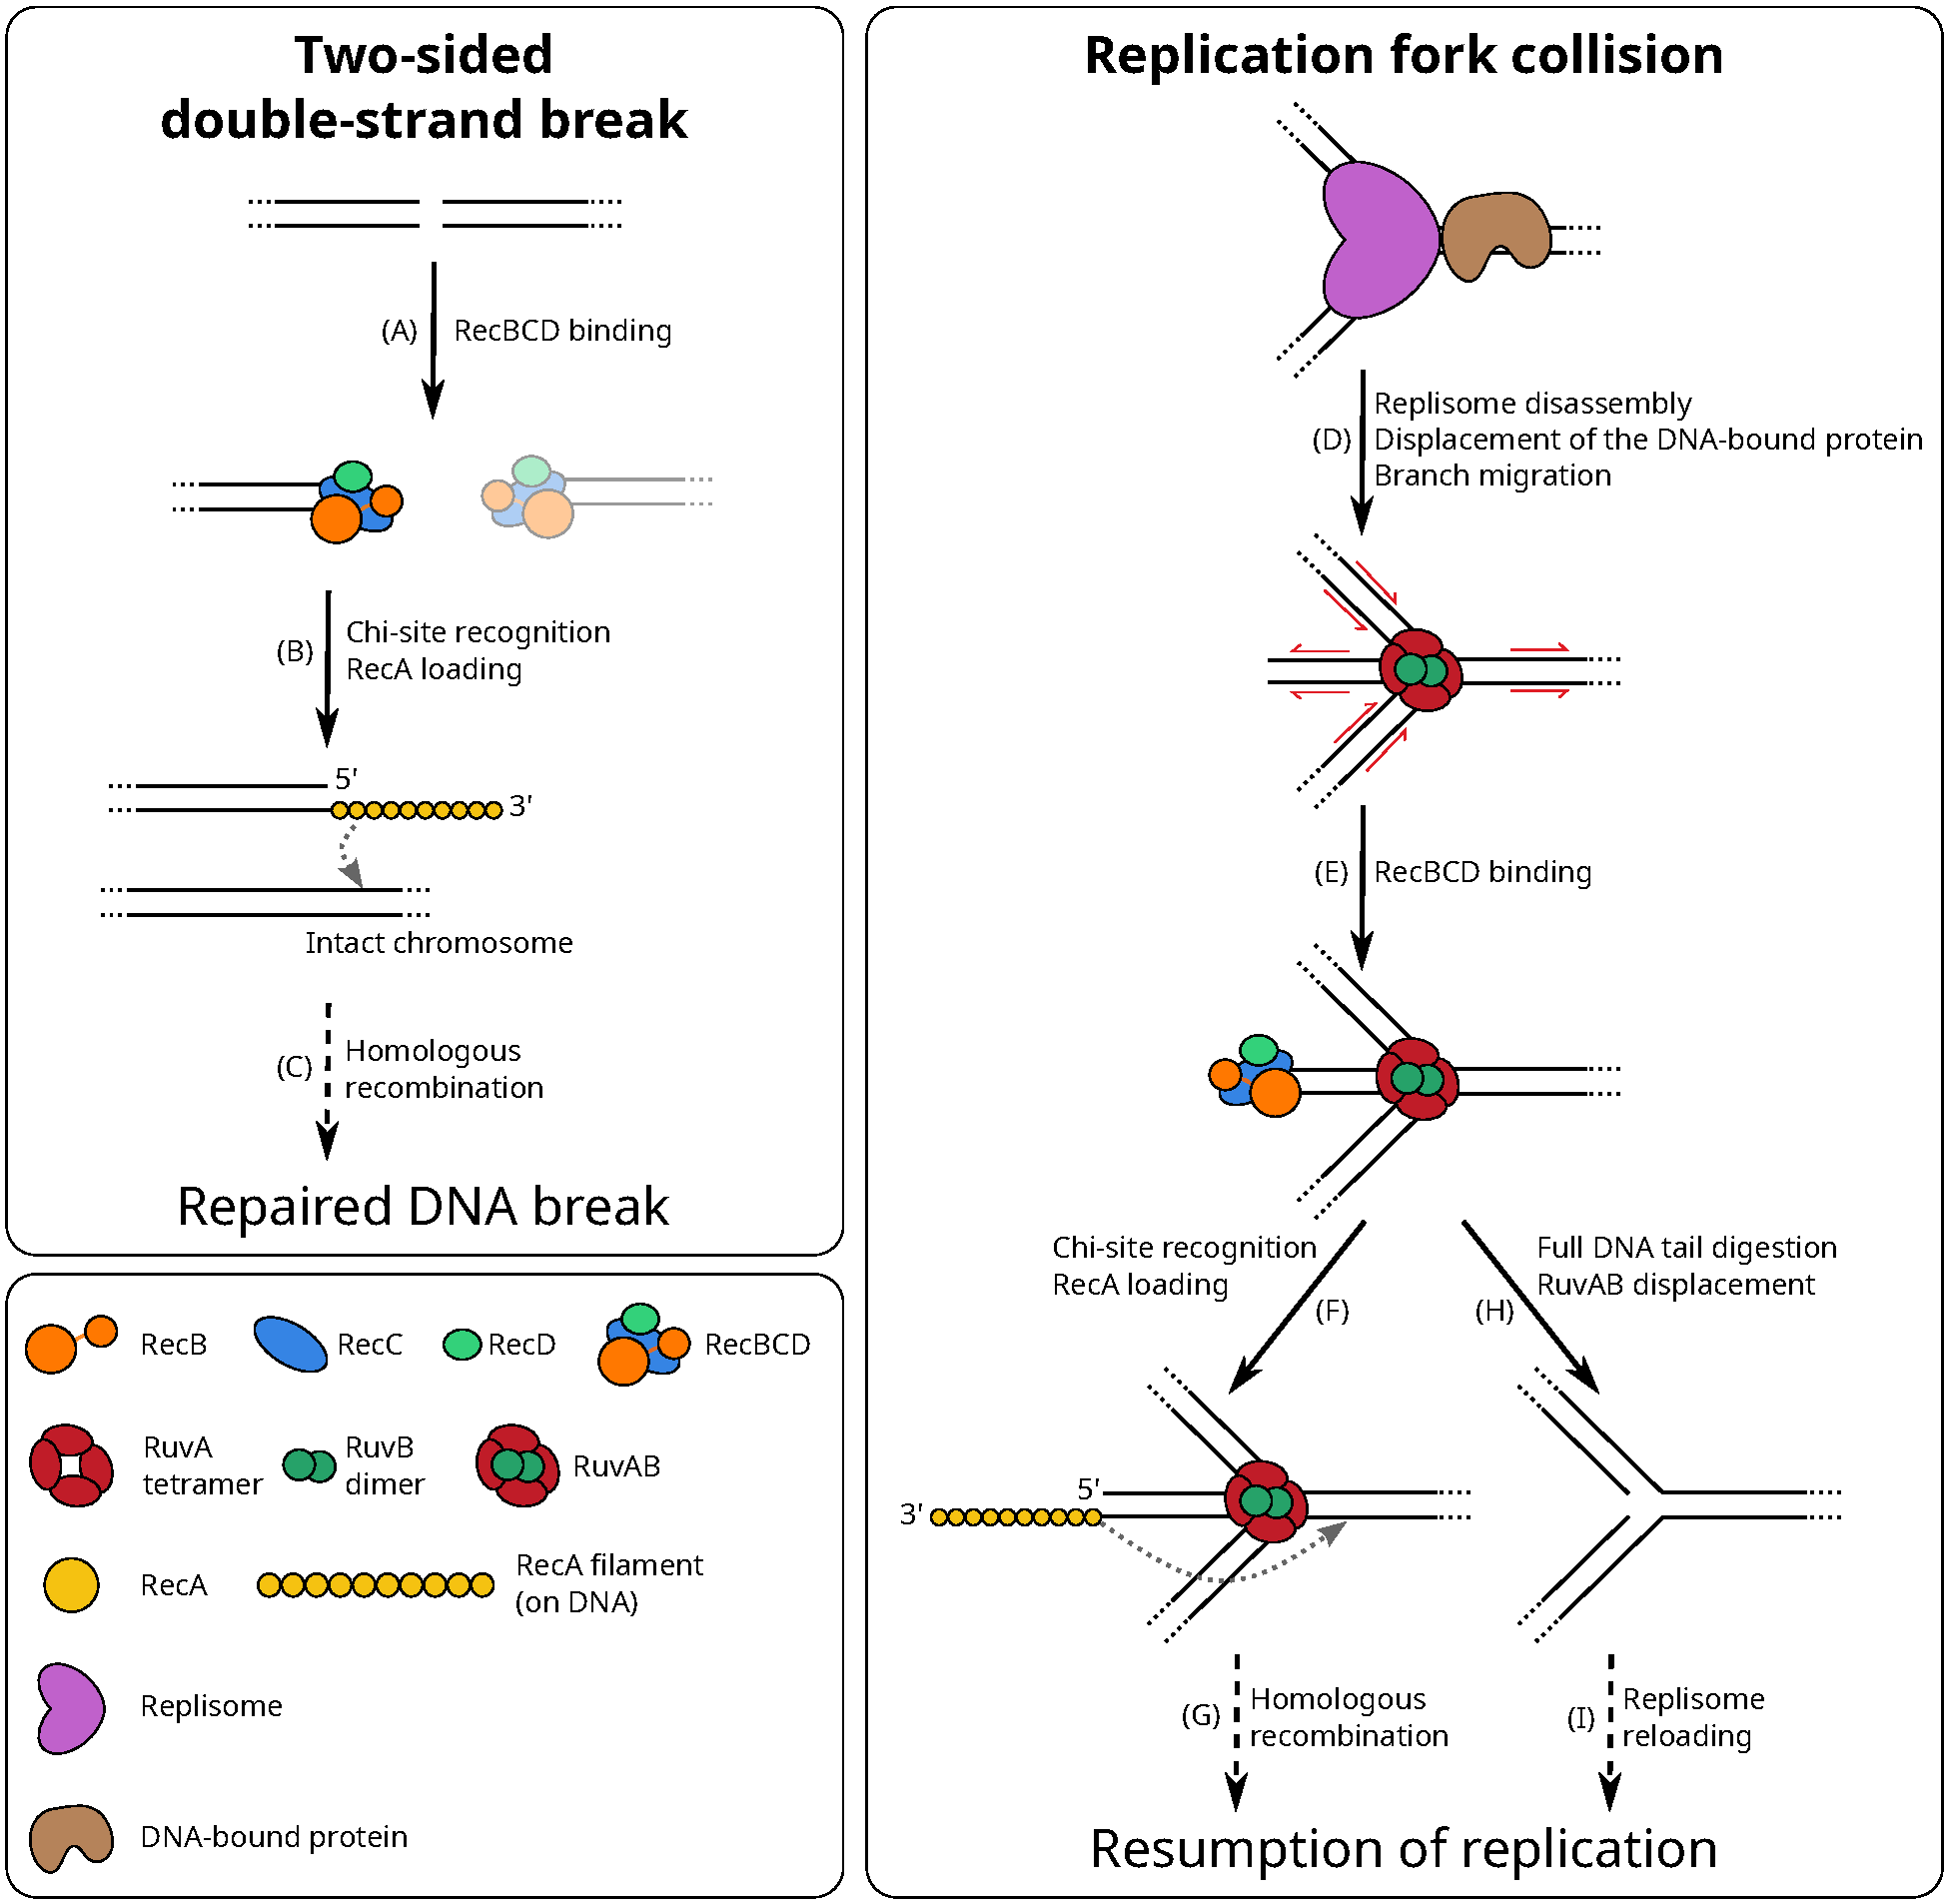
\includegraphics[width=.8\textwidth]{Figures/DSB_scheme.pdf}
    \caption{Double-strand break repair by RecBCD in the case of a two-sided break (left panel), and in the case of replication fork collision (right panel).}
    \label{Fig:DSB_scheme}
\end{figure*}


% DSBs can occur through different processes, and isolated instances are “easy” to deal with
% Review litt on endogenous damage? Michel & Leach papers
% Try to paint a picture of DSB repair that’s more complete than just “clean breaks” (i.e. include fork reversals)
% This could make for a good intro figure, e.g. 2 “simple cases”: fork reversal due to obstacle on the DNA, and clean break (because of UV, nuclease,…). This figure shouldn’t mention cipro/gyrase, because we don't really know what happens there.
% Emphasise that fork reversals are easier (and faster) to deal with, because of dsDNA digestion, or because the homologous sequence is very close



% Antibiotics such as ciprofloxacin can cause massive amounts of damage
% How does the cell deal with that?
% We use different antibiotic concentrations to see the difference between low and high amounts of damage
% We look at our metrics over time to see how the damage is dealt with
% We use mutants to assess the importance of different parts of the repair mechanism


% In this paper, we aim to give more insight into specific steps of DSB repair
% Mechanism of ciprofloxacin DSB generation
% RecBCD binding time
% What happens when damage is too extensive to be repaired






